\let\negmedspace\undefined
\let\negthickspace\undefined
\documentclass[journal]{IEEEtran}
\usepackage[a5paper, margin=10mm, onecolumn]{geometry}
%\usepackage{lmodern} % Ensure lmodern is loaded for pdflatex
\usepackage{tfrupee} % Include tfrupee package

\setlength{\headheight}{1cm} % Set the height of the header box
\setlength{\headsep}{0mm}     % Set the distance between the header box and the top of the text

\usepackage{gvv-book}
\usepackage{gvv}
\usepackage{cite}
\usepackage{amsmath,amssymb,amsfonts,amsthm}
\usepackage{algorithmic}
\usepackage{graphicx}
\usepackage{textcomp}
\usepackage{xcolor}
\usepackage{txfonts}
\usepackage{listings}
\usepackage{enumitem}
\usepackage{mathtools}
\usepackage{gensymb}
\usepackage{comment}
\usepackage[breaklinks=true]{hyperref}
\usepackage{tkz-euclide} 
\usepackage{listings}
\def\inputGnumericTable{}                                 
\usepackage[latin1]{inputenc}                                
\usepackage{color}                                            
\usepackage{array}                                            
\usepackage{longtable}                                       
\usepackage{calc}                                             
\usepackage{multirow}                                         
\usepackage{hhline}                                           
\usepackage{ifthen}                                           
\usepackage{lscape}
\begin{document}

\bibliographystyle{IEEEtran}
\vspace{3cm}

\title{1.6.27}
\author{AI25BTECH11012 - GARIGE UNNATHI}
% \maketitle
% \newpage
% \bigskip
{\let\newpage\relax\maketitle}


\renewcommand{\thefigure}{\theenumi}
\renewcommand{\thetable}{\theenumi}
\setlength{\intextsep}{10pt} % Space between text and floats


\numberwithin{equation}{enumi}
\numberwithin{figure}{enumi}
\renewcommand{\thetable}{\theenumi}


\textbf{Question}:\\
Prove that the three points $\vec{A}$ (-4,6,10) , $\vec{B}$ (2,4,6) and $\vec{C}$ (14,0,-2) are collinear.
\\
\textbf{Solution: }

 \begin{table}[h!]    
      \centering
      

      \caption{Variables Used}
      \label{}
    \end{table}

 If ABC are collinear , then the matrix should have rank 1.
 \begin{align*}
{(\vec{B} - \vec{A} \quad \vec{C} - \vec{A})}^T
\end{align*}


\begin{align}
    {(\vec{B} - \vec{A} \quad \vec{C} - \vec{A})}^T =  \myvec{
6 & -2 & -4 \\
18 & -6 & -12 
}
\end{align}


\begin{align}
    R_2 = R_2 - 3R_1
\end{align}


\begin{align}
     \myvec{
6 & -2 & -4 \\
0 & 0 & 0 
}
\end{align}

Since all the elements of $R_2$ are zero, the rank of the matrix is one.

Hence ABC are collinear points.

\begin{figure}[h!]
   \centering
   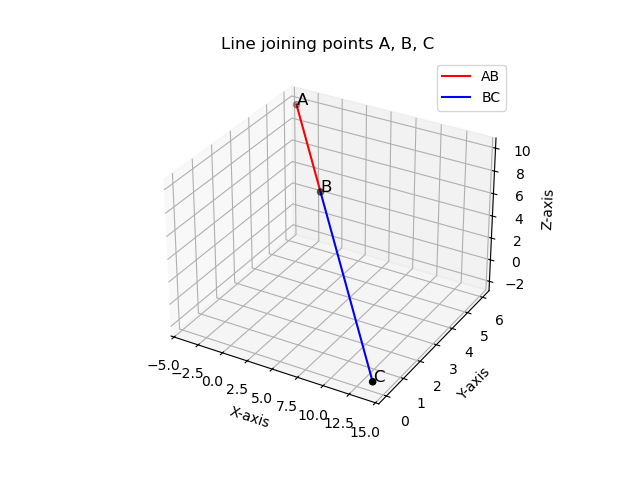
\includegraphics[width=0.7\linewidth]{/Users/unnathi/Documents/ee1030-2025/ai25btech11012/matgeo/1.6.27/figs/figs.png}
   \caption{}
   \label{stemplot}
\end{figure}









\end{document}


